228. \begin{figure}[ht!]
\center{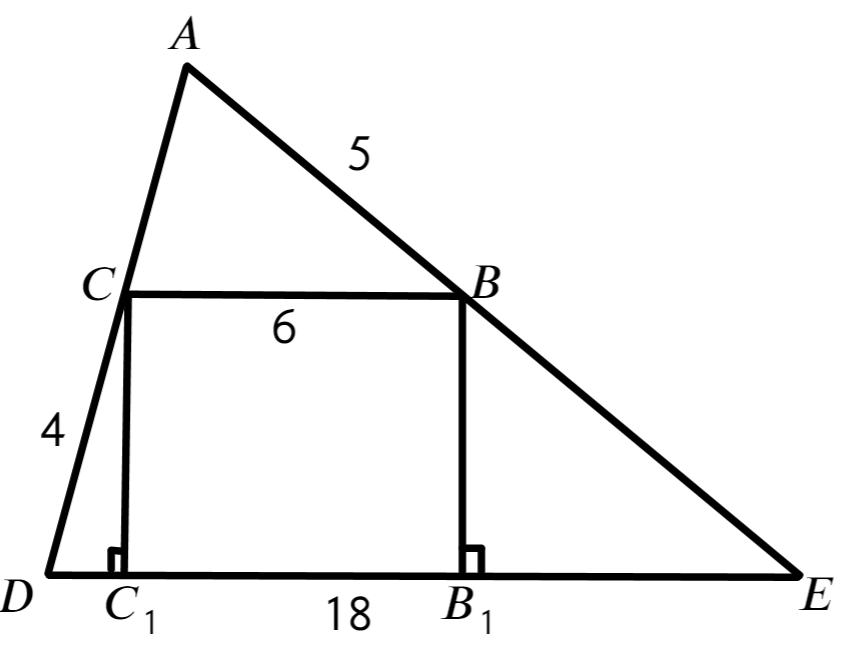
\includegraphics[scale=0.35]{g8-228.png}}
\end{figure}\\
Треугольники $ADE$ и $ACB$ подобны по двум углам (соответственным при параллельных прямых $BC$ и $DE$). Коэффициент подобия равен $\cfrac{DE}{BC}=\cfrac{18}{6}=3.$ Значит, $AE=3AB=3\cdot5=15,$ откуда $BE=15-5=10.$ Опустим в трапеции высоты $CC_1$ и $BB_1.$ Пусть $DC_1=x,$ тогда $B_1E=18-x-6=12-x.$ Выразив квадрат высоты трапеции по теореме Пифагора для треугольников $DCC_1$ и $EBB_1,$ получим равенства $h^2=16-x^2=100-(12-x)^2,$ поэтому $16-x^2=100-144+24x-x^2,\ 24x=60,\ x=\cfrac{5}{2}.$ Тогда $h^2=16-\left(\cfrac{5}{2}
ight)^2=\cfrac{39}{4},\ h=\cfrac{\sqrt{39}}{2}.$ Таким образом, $P=4+6+10+18=38,\ S=\cfrac{\sqrt{39}}{2}\cdot\cfrac{6+18}{2}=6\sqrt{39}.$\\
